
 \frame{
  \frametitle{In the dark ages...}
         	\begin{center}
  			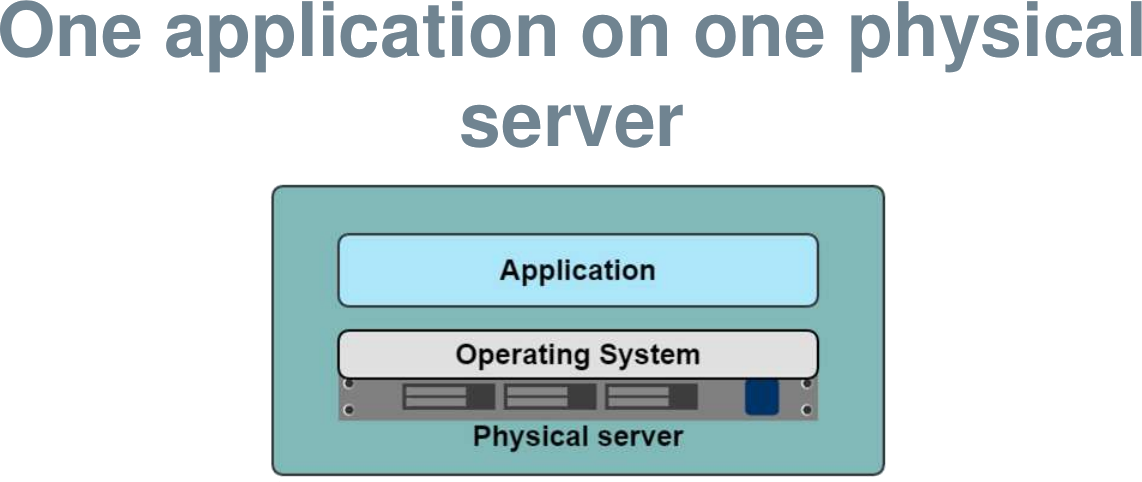
\includegraphics[width=0.80\columnwidth]{./Figure/singleapp}\\
  		\end{center} 
   \begin{columns}[T] % align columns		
   \begin{column}{.40\textwidth}   				
   \begin{itemize}
  		\item Wasted resources;
  		\item Difficult to migrate;
  		\item Difficult to scale;  
  \end{itemize}
\end{column}%
   \hfill%
   \begin{column}{0.35\textwidth}
      \begin{itemize}
     	\item Slow deployment rate;
  	 	\item Huge costs.
      \end{itemize}
   \end{column}%
   \end{columns}

  } 
  
  \frame{
  \frametitle{Virtual machines (VM)  and containers provide}  \vspace{0.25cm}  
 \begin{itemize}
 \item Better resource utilization:\vspace{0.15cm}
	\centerline{\color{NavyBlue}\emph{Multiple  VMs/containers can run on the same physical machine}}\vspace{0.2cm}
 \item Better service scalability:\vspace{0.15cm}
 \centerline{\color{NavyBlue}\emph{New VMs/containers associated with a service can be started when needed}}\vspace{0.2cm}
 \item Better level of portability and adaptability:\vspace{0.15cm}
  \centerline{\color{NavyBlue}\emph{VMs/containers can easily migrate from a server to another}}\vspace{0.2cm}
  \item Higher reproducibility level:\vspace{0.15cm}
    \centerline{\color{NavyBlue}\emph{Using VMs/containers we can freeze the version of tools, libraries ...}}
\end{itemize}\vspace{-0.15cm}
\begin{center}
  			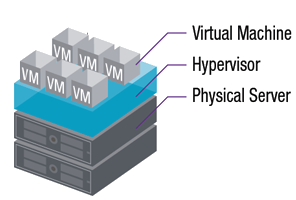
\includegraphics[width=0.35\columnwidth]{./Figure/vm3}~~~~
  			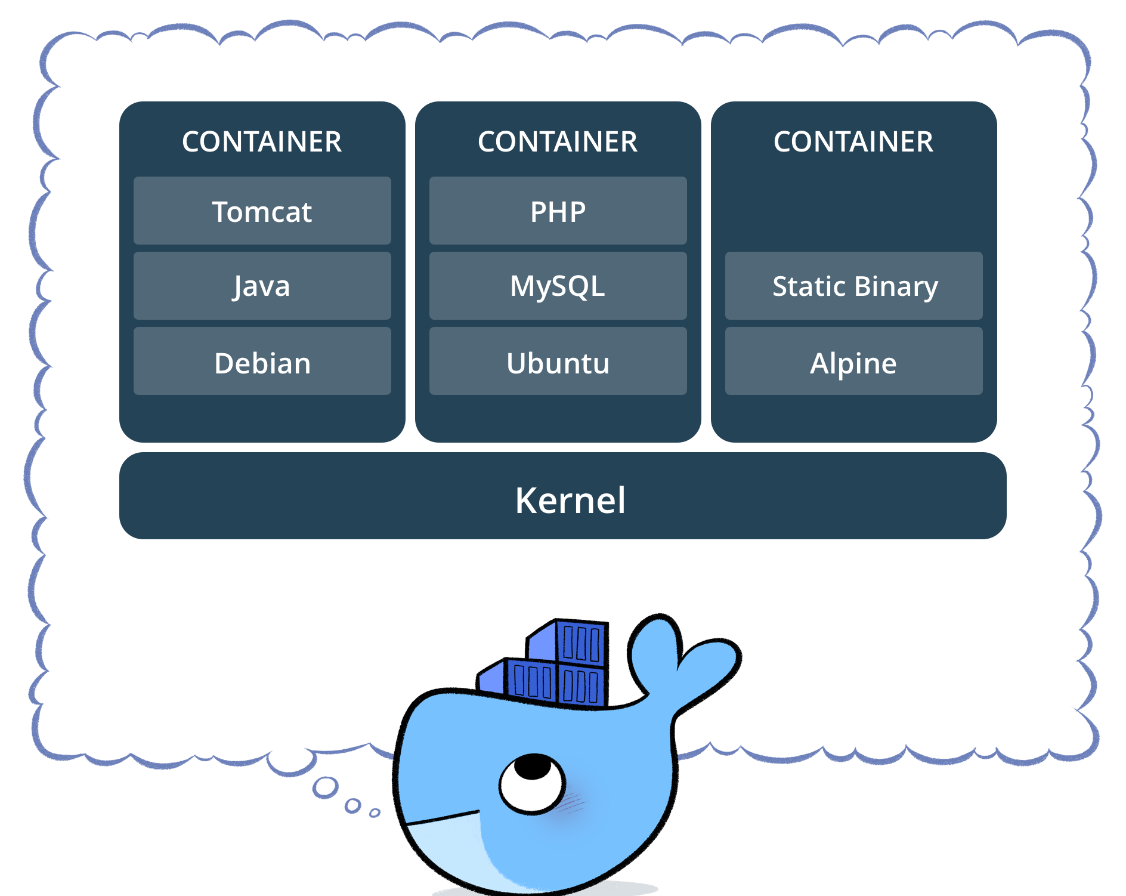
\includegraphics[width=0.27\columnwidth]{./Figure/dockerGen}
  		\end{center} 
}
  
  
  
  
 \frame{
  \frametitle {Containers VS Virtual Machines}
 % \vspace{0.3cm}
  % \textbf{\color{NavyBlue}Containers VS VM}\vspace{-0.5cm}
  \begin{columns}[T] % align columns
  \begin{column}{.50\textwidth}
  \vspace{0.8cm}
		\begin{center}
  			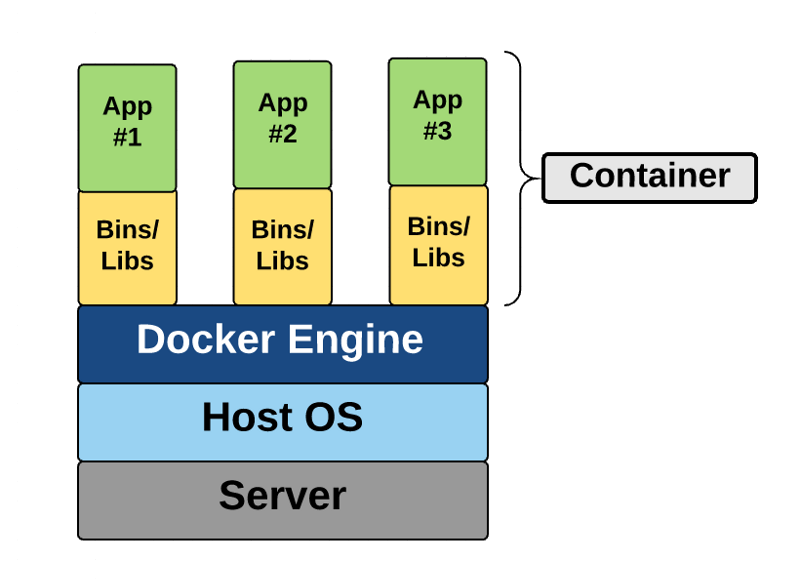
\includegraphics[width=1.00\columnwidth]{./Figure/Container}\\
  		\end{center}\vspace{-0.4cm}
  		Containers are an application level construct.
   \end{column}%
   \hfill%
   \begin{column}{0.50\textwidth}
     	\begin{center}
  			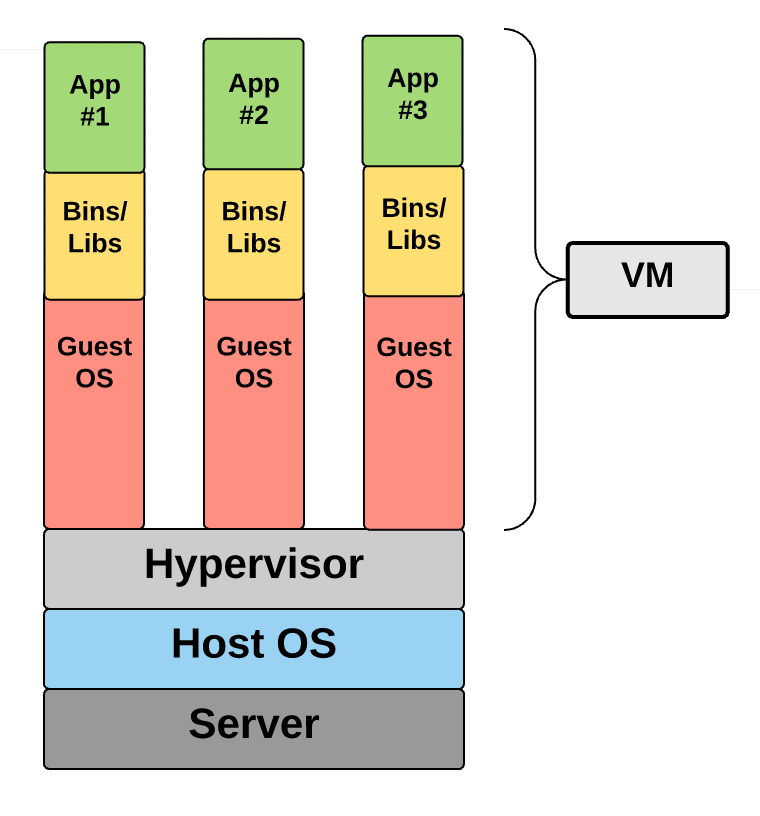
\includegraphics[width=1.00\columnwidth]{./Figure/vm2}\\
  		\end{center}
  	\vspace{-0.4cm}VMs are an infrastructure level construct. 
   \end{column}%
   \end{columns}
  }   
  
  
  
  \frame{
  \frametitle {Containers VS Virtual Machines}
 	\begin{center}
  			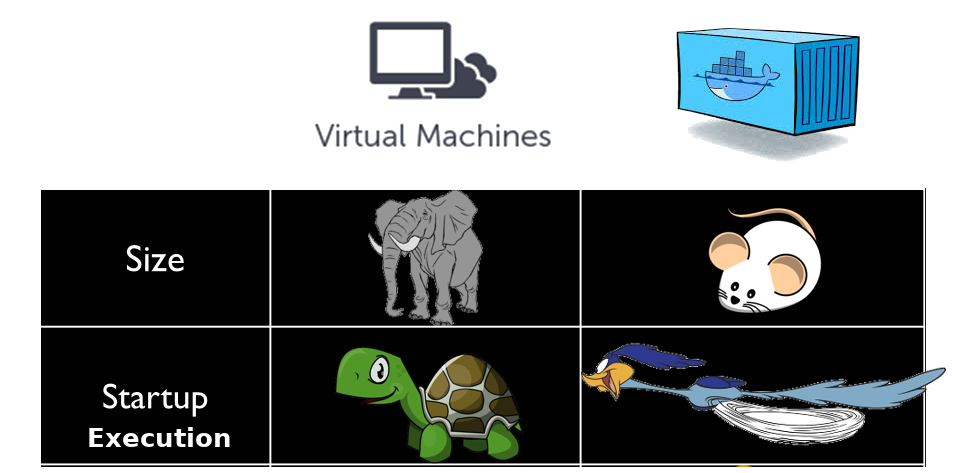
\includegraphics[width=0.90\columnwidth]{./Figure/ContainersVSVM}\\
  		\end{center}
  		
  \textbf{\color{NavyBlue}\emph{In Containers the sharing of the same OS Kernel with the real machine reduces the application portability, but ....}	}	
  } 


\frame{
\frametitle{Container, VM and real server: a comparison}
In [1] a comparison among physical server, KVM, and Docker is reported.

     	\begin{center}
  			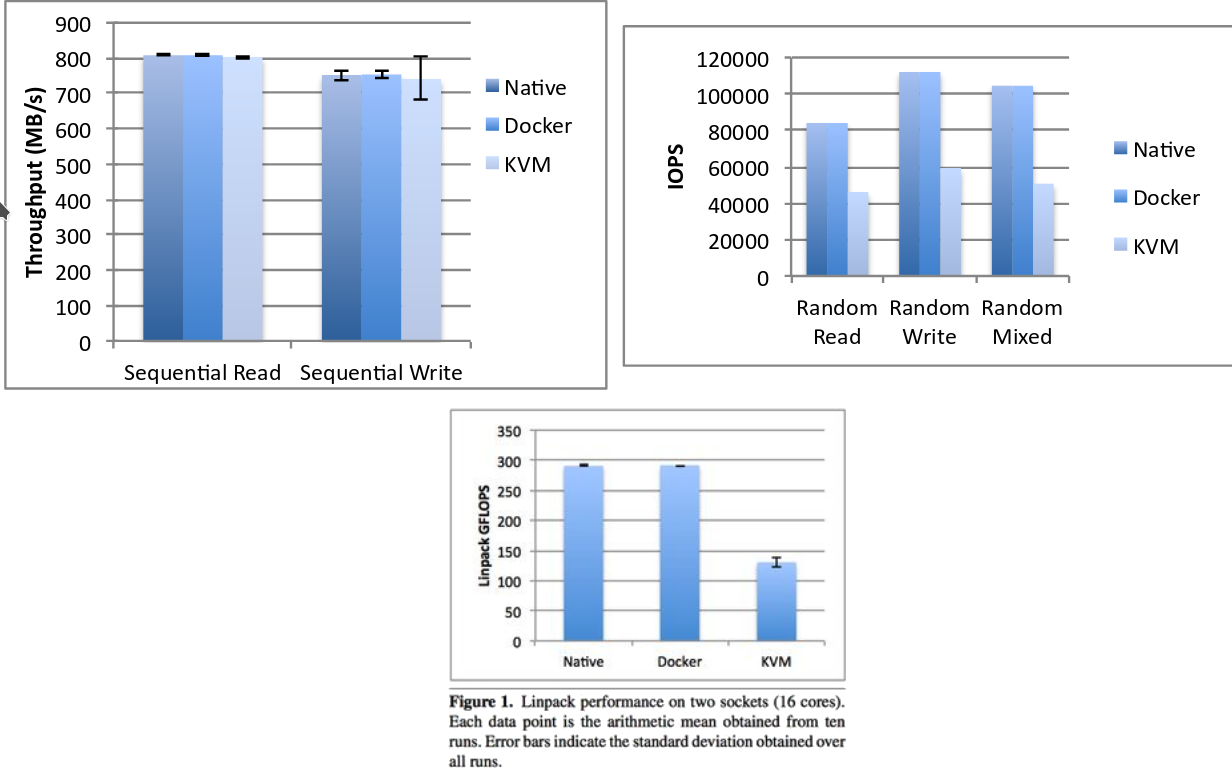
\includegraphics[width=0.90\columnwidth]{./Figure/benchmark}
  		\end{center}  
{\tiny
[1] W. Felter, A. Ferreira, R. Rajamony and J. Rubio, \emph{\textbf{An updated performance comparison of virtual machines and Linux containers}}, 2015 IEEE International Symposium on Performance Analysis of Systems and Software (ISPASS), Philadelphia, PA, 2015, pp. 171-172.

}
} 

  
  
\frame{
  \frametitle {Docker project}
  
  
  
  \begin{columns}[T] % align columns
  \begin{column}{.55\textwidth}
  	\begin{itemize}
 		\item Docker is an open-source project based on Linux containers.
 	\vspace{0.3cm}
 		\item Others Linux container technologies include Solaris Zones, BSD jails, and LXC, which have been around for many years.
 		 	\vspace{0.3cm}	
      	\end{itemize}
   \end{column}%
   \hfill%
   \begin{column}{0.45\textwidth}
   \vspace{-1.2cm}
     	\begin{center}
  			
\includegraphics[width=1.05\columnwidth]{./Figure/Docker}\\
  		\end{center}
   \end{column}%
   \end{columns}
   \vspace{0.8cm}
   \centerline{\Huge \color{NavyBlue} \textbf{\emph{Why to choose Docker?}}}
  } 
  
\frame{
  \frametitle {Why to use Docker?}
  
    \begin{columns}[T] % align columns
  \begin{column}{.65\textwidth}
  	\begin{itemize}
	\item  \textbf{\color{NavyBlue} Ease of use:} Docker has made it much easier for anyone to take advantage of containers in order to quickly build and test portable applications; \vspace{0.3cm}	
	
	\item  \textbf{\color{NavyBlue} Speed:} Docker containers are very lightweight and fast.
	\vspace{0.3cm}	
	\item \textbf{\color{NavyBlue}Docker Hub:} Docker users also benefit from the increasingly rich repository of Docker Hub, which you can think of as an ``app store for Docker images''; 
	\vspace{0.3cm}	
	\item \textbf{\color{NavyBlue}Modularity and Scalability:} Docker makes it easy to break out your application's functionality into individual containers.
  	\end{itemize}
   \end{column}%
   \hfill%
   \begin{column}{0.35\textwidth}
     	\begin{center}
  			
\includegraphics[width=1.05\columnwidth]{./Figure/Docker}\\
  		\end{center}
   \end{column}%
   \end{columns}
  } 
    


  \frame{
  \frametitle{Docker family picture} \vspace{0.3cm}
  \begin{center}
  			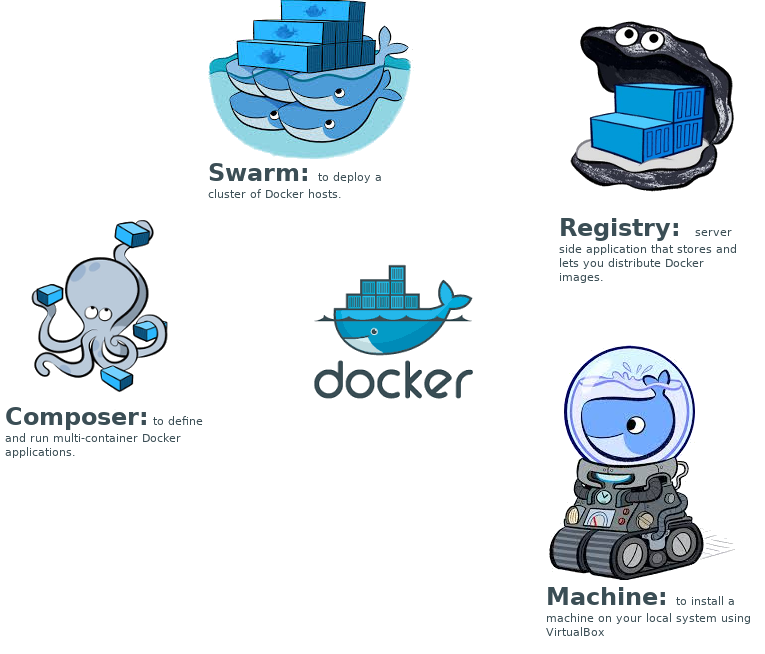
\includegraphics[width=0.77\columnwidth]{./Figure/family2}\\
  		\end{center} 
 } 	

 		
\frame{
\frametitle{Docker basics} 
\vspace{0.2cm}
\begin{itemize}
\item \textbf{\color{NavyBlue}\emph{Image}} is an executable package that includes everything needed to run an application (i.e. its code,  libraries, environment variables, and configuration files);\vspace{0.2cm}
\item \textbf{\color{NavyBlue}\emph{Container}} is a run-time instance of an image;\vspace{0.2cm}
\item \textbf{\color{NavyBlue}\emph{Volume}} is used to  share files from the host machine to containers.
\end{itemize}
\vspace{0.2cm}
  \begin{center}
  			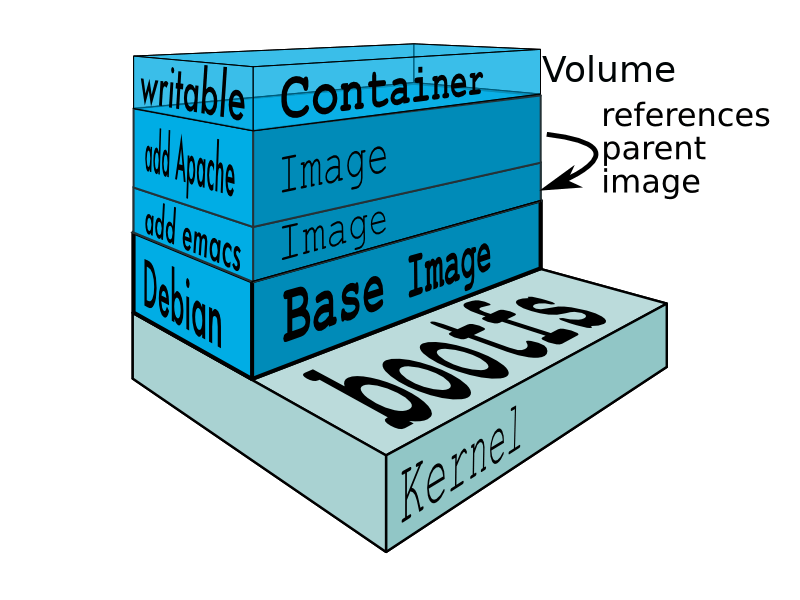
\includegraphics[width=0.55\columnwidth]{./Figure/exec}\\
  		\end{center} 

}

\frame{
\frametitle{Docker architecture} 
  \begin{center}
  			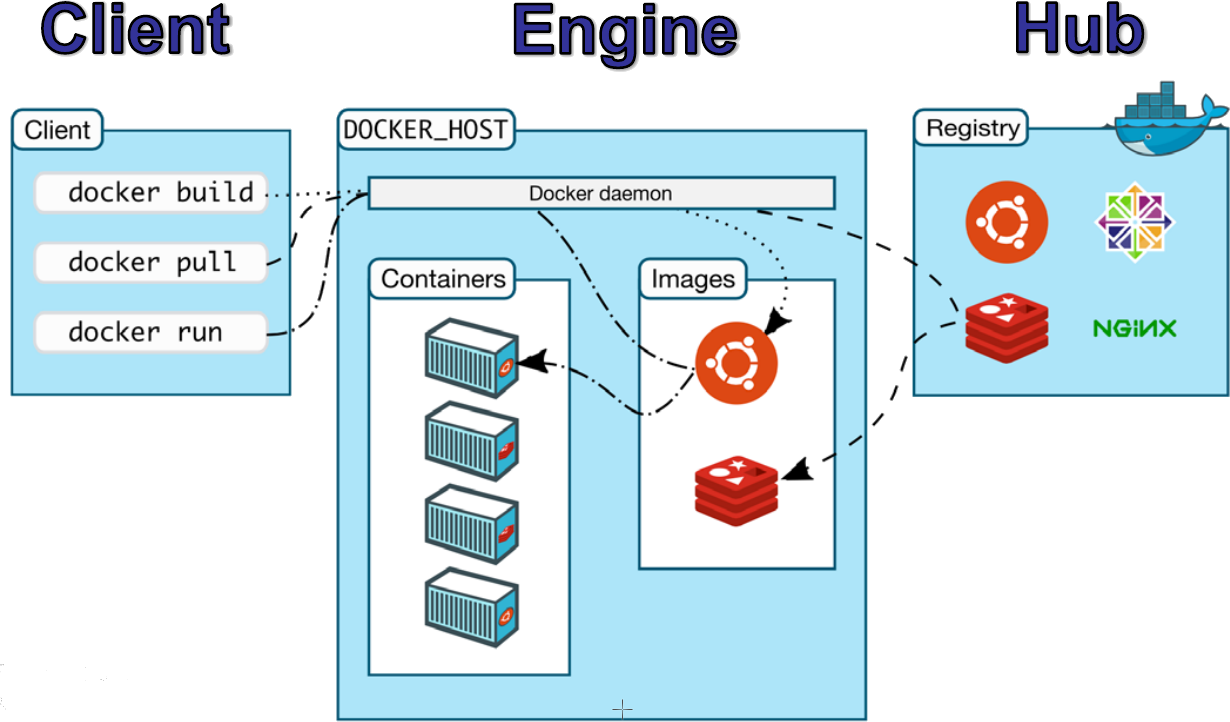
\includegraphics[width=1.02\columnwidth]{./Figure/arc}\\
  		\end{center} 

} 	
 
 \frame{
\frametitle{Docker client} 
    \begin{columns}[T] % align columns
  \begin{column}{.65\textwidth}
  \vspace{2.5cm}
  	\begin{itemize}
	\item It provides  an interface for users;\vspace{0.3cm}	
	\item It is cross Platform:  OSX,  Windows and  Linux;\vspace{0.3cm}	
	\item It allows  Local and Remote Execution.\vspace{0.3cm}	
  	\end{itemize}
   \end{column}%
   \hfill%
   \begin{column}{0.35\textwidth}
     	\begin{center}
  			
\includegraphics[width=1.00\columnwidth]{./Figure/Client}
  		\end{center}
   \end{column}%
   \end{columns}
  } 
  
   \frame{
\frametitle{Docker engine} 
    \begin{columns}[T] % align columns
  \begin{column}{.65\textwidth}
  \vspace{0.5cm}
  	\begin{itemize}
	\item It executes the commands received by the Docker Client;\vspace{0.3cm}
	\item It builds and menages images;	\vspace{0.3cm}	
	\item It creates and menages the Containers.\vspace{0.3cm}	
  	\end{itemize}
   \end{column}%
   \hfill%
   \begin{column}{0.38\textwidth}
     	\begin{center}
  			
\includegraphics[width=1.00\columnwidth]{./Figure/engine}
  		\end{center}
   \end{column}%
   \end{columns}
  } 